\begin{frame}
\frametitle{Microreactors}
\begin{columns}
	\column[t]{5cm}
	\begin{itemize}
		\item Description of microreactors
	\end{itemize}

    \column[t]{5cm}
	\begin{figure}[htbp!]
		\begin{center}
			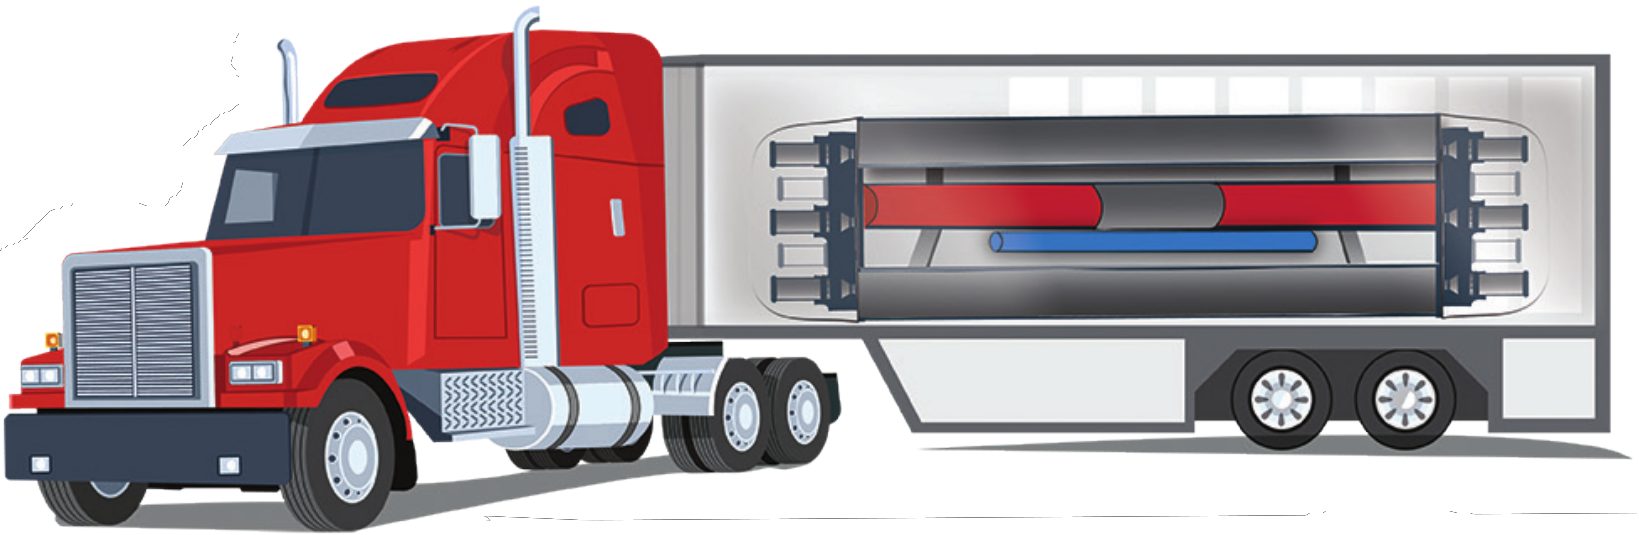
\includegraphics[height=6.2cm]{images/microreactor}
		\end{center}
		\caption{.}
	\end{figure}
\end{columns}
\end{frame}

% should i give a description of different designs??